%https://www.overleaf.com/learn/latex/Creating_a_document_in_LaTeX
\documentclass[12pt]{report}
\usepackage{graphicx}

\title{CS 440: This Maze is on Fire}
\author{Steven Nguyen \& Kyra Kennedy}
\date{19 February 2021}

\graphicspath{ {./test_results/} }
\renewcommand{\arraystretch}{1.25}

\begin{document}

\begin{titlepage}
\maketitle
\end{titlepage}

\section{Abstract}
In the first part of the project, we demonstrate generating 2D mazes on command line and demonstrate navigating through the mazes using DFS, BFS, and A*.\\
In the second part of the project, we demonstrate again navigating, however, there will be a special barrier randomly placed in the maze that expands randomly through neighboring cells.

\section{Academic Integrity}
It was agreed from when we first started that Steven Nguyen would handle problems 1, 2, 3, 4, 6, and 8 while Kyra Kennedy worked on strategy 3 and problems 5 and 7. Both members assisted in this write up.\\
I, Steven Nguyen, have not copied our code or taken from online or another student's work.\\
I, Kyra Kennedy, have not copied our code or taken from online or another student's work.

\section{Problem 1}
Please see the attached file, \emph{maze.py}, for both generating the maze structure and for filling the structure given parameters.

\break
\section{Problem 2}
Please see the attached file, \emph{dfs.py}, for the implementation of DFS.\\
For finding if a point is reachable from the other, DFS is better than BFS in this case because while both searches find the path in at most the same amount of steps and at least the same amount of steps, DFS uses a much less amount of memory while searching.\\
\begin{figure}[h]
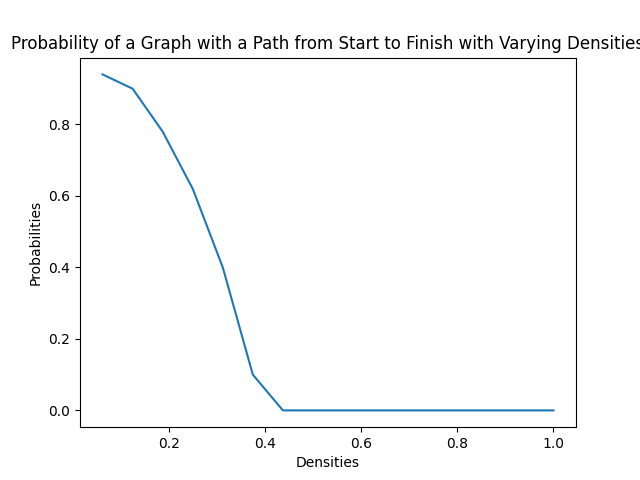
\includegraphics[width=\textwidth]{Probability of a Graph with Path vs Density.png}
\caption{Compares the probability that a graph has at least one valid path from start to finish using Manhattan Distance in random 100 by 100 mazes vs density}
\label{Probability of a Graph with a Complete Path vs Density}
\end{figure}\\
We determined that as density increases, the probability that a maze has at least one valid path is lowered.

\break
\section{Problem 3}
Please see the attached files, \emph{bfs.py} and \emph{a.py}, for the implementations of BFS and A*.\\
In our project, when plotting \emph{the number of nodes explored by BFS} and \emph{the number of nodes explored by A*} vs \emph{the density of the generated maze}.\\
\begin{figure}[h]
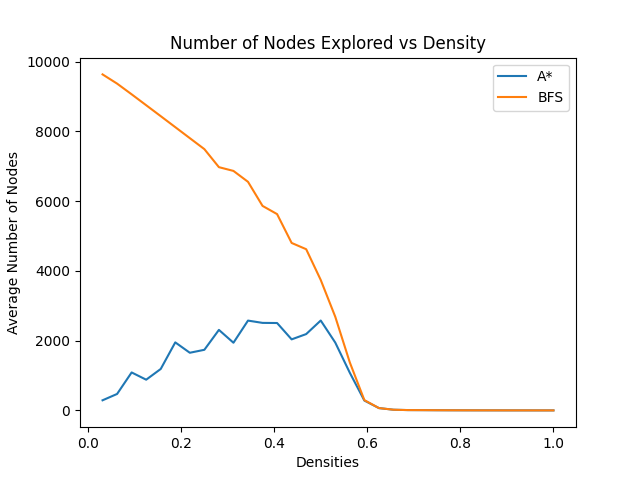
\includegraphics[width=\textwidth]{Number of Nodes Explored vs Density.png}
\caption{Compares the average number of nodes explored by Euclidean Distance in random 100 by 100 mazes vs density for both A* and BFS}
\label{Number of Nodes Explored vs Density}
\end{figure}\\
Up until around .5 density, the average number of explored nodes in A* increases because longer paths must be generated with more barrier. Then after around .5, there are significantly more mazes that do not have a valid path from start to finish, so less nodes are explored because both there are less explorable nodes and less paths. \\
For BFS, because the mazes are designed so the start is on the top left and end is on the bottom right, BFS will search almost all cells in the maze and will end up searching much more cells than A* when the density is low.

\break
\section{Problem 4}
\begin{figure}[h]
\begin{center}
\begin{tabular}[c]{ |c|c| }
\hline
\multicolumn{2}{ |c| }{Max Size Maze for Search Algorithms}\\
\hline
Search Algorithm & Max Size\\
\hline
DFS & 1300 by 1300\\
BFS & 3300 by 3300\\
A* & 1500 by 1500\\
\hline
\end{tabular}
\end{center}
\caption{Within 60.00 seconds, at 0.3 Density, DFS can search a 1300 by 1300 maze, BFS can search a 3300 by 3300 maze, and A* can search a 1500 by 1500 maze.}
\label{Probability of a Graph with a Complete Path vs Density}
\end{figure}
A* is slow because it is spending too many operations finding which of its neighbors is closer to the end whenever scanning each cell. DFS is slow probably because the start and end cells are not randomly placed and DFS, in our case, scans neighbors starting from the top in a clockwise direction. So, DFS spreads in the downward-left direction while the goal is always in the downward-right direction.

\section{Problem 5}
For strategy 3, named Too H.A.W.T. to Handel, where H.A.W.T stands for Hop Along Without Threat. For this strategy, at each step the agent checks its immediate neighbors to its north, south, east, and west. If one of them is on fire, a new path is computed, otherwise it continues on the last path it computed. By doing so, a new path doesn't have to be created at every turn, such as in strategy 2, but still allows for re-computation, unlike strategy 1.\\
This accounts for the unknown future in that when fire is nearby, it acknowledges that it poses a threat in the near future and computes a new path to now avoid it. In this way, the strategy is more aware of where the fire is and how it should move around it.

\break
\section{Problem 6}
[Insert plot for success rates here]
do be do be do ba

\section{Problem 7}
With unlimited computational resources, strategy 3 could be improved with a more Stochastic model. This would be able to calculate an indepth game tree for any size maze and allow the agent to find the most efficient path even when accounting for future fire spread. Since the code for this was gone over in recitation, it wasn't chosen for strategy 3, but its inclusion would improve the code's ability to plan for the future spread by analyzing all possible paths of the fire.

\section{Problem 8}
With a limited time between moves, we would reduce the computation by reducing the length of the path used in the prediction e.g., pathfind to just a bit after the fire rather than all the way to the end; and by reducing how many paths are searched when predicting, such as paths that go in the opposite direction of the goal.

\end{document}